% GWGEN chapter

\Chapter{GWGEN v1.0}{A globally calibrated scheme for generating daily meteorology from monthly statistics}

\label{chp:gwgen}

\begin{refsection}
	
\begin{abstract}
	While a wide range of earth system processes occur at daily and even sub-daily timescales, many global vegetation and other terrestrial dynamics models historically used monthly meteorological forcing, both to reduce computational demand and because global datasets were lacking. Recently, dynamic land surface modeling has moved towards resolving daily and subdaily processes, and global datasets containg daily or sub-daily meteorology have become available. These meteorological datasets, however, cover only the instrumental era of the last ca. 100 years at best, are subject to considerable uncertainty, and represent extremely large data files with associated computational costs of data input/output and file transfer. For periods before the recent past or into the future, global meteorological forcing can be provided by climate model output, but the quality of these data at high temporal resolution is low, particularly e.g., with daily precipitation frequency and amount. Here we present ARVE-WGEN, a globally applicable statistical weather generator for the temporal downscaling of monthly climatology to daily meteorology. Our weather generator is parameterized using a global meteorological database and simulates daily values of five common daily weather variables: minimum and maximum temperature, precipitation, cloud cover, and windspeed. ARVE-WGEN is lightweight, modular, and requires a minimal set of monthly mean variables as input. The weather generator may be used in a range of applications, for example, in global vegetation, crop, erosion, or hydrological models.
\end{abstract}

%----------------------------------------------------------------------------------------
%	SECTION 1
%----------------------------------------------------------------------------------------
\section{Introduction} \label{sec:gwgen-intro}

The development of the first global vegetation models in the 1970’s \citep[e.g.][]{Lieth1975} brought about the demand for meteorological forcing datasets with global extent and relatively high spatial resolution, e.g., ~1x1°. While a global weather station-based monthly climate dataset was available at this time \citep{WalterLieth1967}, limitations in computers and data storage allowed only the simplest treatment of these data. The first global simulations of the net primary productivity of the terrestrial biosphere \citep{Lieth1975}, thus used rasterized polygons of annual meteorological variables that had been crudely interpolated from the station-based climatology. A decade later saw the development of better computers and more sophisticated global vegetation models \citep{PrenticeCramerHarrisonEtAl1992, Prentice1989} that recognized the need for forcing at a sub-annual timestep and development of these models was done in parallel with the first global, gridded high resolution (0.5°) monthly climatology \citep{LeemansCramer1991}. At the time, monthly meteorological data was the only feasible global data that could be produced, in terms of the raw station data available to feed the interpolation process, the processing time required to produce gridded maps, and the data storage and transfer capabilities of contemporary computer systems and networks. Global gridded monthly climate data became the standard for not only large-extent vegetation modeling \citep{HaxeltinePrentice1996a, HaxeltinePrenticeCreswell1996,KaplanBigelowPrenticeEtAl2003, KucharikFoleyDelireEtAl2000, WoodwardSmithEmanuel1995}, but also for a wide range of studies on biodiversity and species distribution \citep[e.g.][]{ElithGrahamAndersonEtAl2006}, vegetation trace gas emissions \citep[e.g.][]{GuentherHewittEricksonEtAl1995}, and even the geographic distribution of human diseases \citep[e.g.][]{BhattGethingBradyEtAl2013}

Over subsequent years, the global gridded monthly climate datasets were improved \citep{NewHulmeJones1999,NewListerHulmeEtAl2002}, developed with very high spatial resolution \citep{HijmansCameronParraEtAl2005}, and expanded beyond climatological mean climate to cover continuous timeseries over decades \citep{HarrisJonesOsbornEtAl2014,MitchellJones2005,NewHulmeJones2000}. The latter was an essential requirement for forcing dynamic global vegetation models (DGVMs) \citep[e.g.][]{SitchSmithPrenticeEtAl2003}. However despite increasing quality, spatial resolution, and temporal extent in these datasets, the basic time step remained monthly, partly for legacy reasons – models had been developed in an earlier era subject to computational limitations and therefore used a monthly timestep for efficiency even if this was no longer strictly a constraint – and partly because of the challenge in developing a global, high-resolution climate dataset with a daily or shorter timestep still presented a major data management challenge.

On the other hand, there was increasing awareness that accurate simulation of many earth surface processes required representation of processes at a shorter-than-monthly timestep. Global simulation of surface hydrology \citep{GertenSchaphoffHaberlandtEtAl2004}, crop growth \citep{BondeauSmithZaehleEtAl2007}, or biogeophysical processes \citep{KrinnerViovyNoblet-DucoudreEtAl2005} needed sub-monthly forcing to produce reliable results. To address this need for better forcing data, two main approaches were taken: either monthly climate data were downscaled online using a stochastic weather generator \citep{PfeifferSpessaKaplan2013}, or a sub-daily, high-resolution, gridded climate timeseries was generated directly by merging high-temporal-resolution reanalysis data (e.g., NCEP, 6h, 2.5°) with high-spatial-resolution monthly climate data (e.g., CRU, 0.5°). The latter process resulted in the CRUNCEP dataset \citep{ViovyCiais2016,WeiLiuHuntzingerEtAl2014}, which, while global, is large even by modern standards (ca. 350 Gb), is not available at spatial resolution greater than 0.5°, and covers only the period 1901-2014.

Forcing data for global vegetation and other models with shorter than monthly resolution at higher spatial resolutions than 0.5°, or for any other period than the last ca. 120 years, e.g., for the future or the more distant past, may therefore only be available through downscaling techniques. One approach to overcome the limitations of currently available datasets could be to use GCM output directly, however, most GCM output currently available does not have greater than 0.5° spatial resolution, with the current generation of GCMs typically approaching ca. 1°x1° degree. Furthermore, there is a general observation that daily meteorology produced by GCMs is not realistic, particularly for precipitation \citep{Dai2006,StephensLEcuyerForbesEtAl2010,SunSolomonDaiEtAl2006}. An alternative approach is, therefore, to perform temporal downscaling on monthly meteorological data using a statistical weather generator.

Statistical weather generators were first developed primarily for crop and hydrological modeling at the field to catchment scale \citep{Richardson1981,WoolhiserPegram1979,WoolhiserRoldan1982}. The weather generator was parameterized using daily meteorological observations at one or more weather stations close to the area of interest, although some attempts were made to generalize the parameterization over larger, sub-continental regions \citep[e.g.][]{Wilks1999a,Wilks1998,WoolhiserRoldan1986}. Locally parameterized weather generators have been applied to a very wide range of studies \citep{Wilks2010,WilksWilby1999}, and enhanced to include additional meteorological variables beyond the original precipitation, temperature, and solar radiation \citep[e.g.][]{ParlangeKatz2000}. Applications of a weather generator at continental to global scales was still limited, however, because of the need to perform local parameterization.

The need to simulate daily meteorology in regions of the world with short, unreliable, or unavailable daily meteorological timeseries brought about the realization that certain features of weather generator parameterization might be generalized across a range of climates \citep{GengAuburn1987,GengDevriesSupit1986}. This ultimately led to the development of globally applicable weather generators \citep{Friend1998}, and their incorporation in DGVMs \citep{BondeauSmithZaehleEtAl2007,GertenSchaphoffHaberlandtEtAl2004,PfeifferSpessaKaplan2013}. The original global parameterization \citep{GengDevriesSupit1986} of these weather generators was, however, limited to seven weather stations, mostly in the temperate latitudes. \cite{Friend1998} does not publish the parameters used in his global weather generator, but we assume these were the same as the original \cite{GengAuburn1987,GengDevriesSupit1986} models. Given the availability of 1) large datasets of daily meteorology, and 2) computers powerful enough to process these data, we therefore decided that it would be valuable to revisit these parameterizations, perform a systematic and quantitative evaluation of the resulting downscaled meteorology, and potentially improve our ability to perform monthly-to-daily downscaling of common meteorological variables with a single, globally applicable parameterization.

In the following sections we describe GWGEN, a weather generator parameterized using more than 50 million daily weather observations, from all continents and latitudes. We demonstrate how updated schemes for simulating precipitation occurrence and amount, and for correcting bias in temperature and wind speed, further improve the quality of the model simulations. We perform an extensive model evaluation and parameter uncertainty analysis in order to settle on a parameter set that provides the most accurate, globally applicable results. We comment on the limitations of the model and priorities for future research. The GWGEN is an open-source, stand-alone model that may be incorporated into any number of models designed to work at global scale, including, e.g., vegetation, hydrology, climatology, and animal distribution models.


\section{Model development}

Our WGEN type weather generator follows the methodology described by \cite{Richardson1981}, the simple method described by \cite{GengDevriesSupit1986}. It uses a second-order Markov chain as described in \cite{Wilks1999} to calculate the precipitation occurrence and a hybrid Gamma-GP distribution \citep{NeykovNeytchevZucchini2014} to estimate the amount. Temperature, cloud cover and wind speed are calculated via cross correlation and depending on the wet/dry-state of the day. An additional quantile-based bias correction for wind speed and minimum temperature improves the simulation results significantly.

In this section, we describe the global weather station database and provide the underlying figures and equations that have been used for the parameterization of GWGEN. A full model description can be found in section \ref{sec:model}.

\subsection{Development of global weather station database}
\begin{figure}
	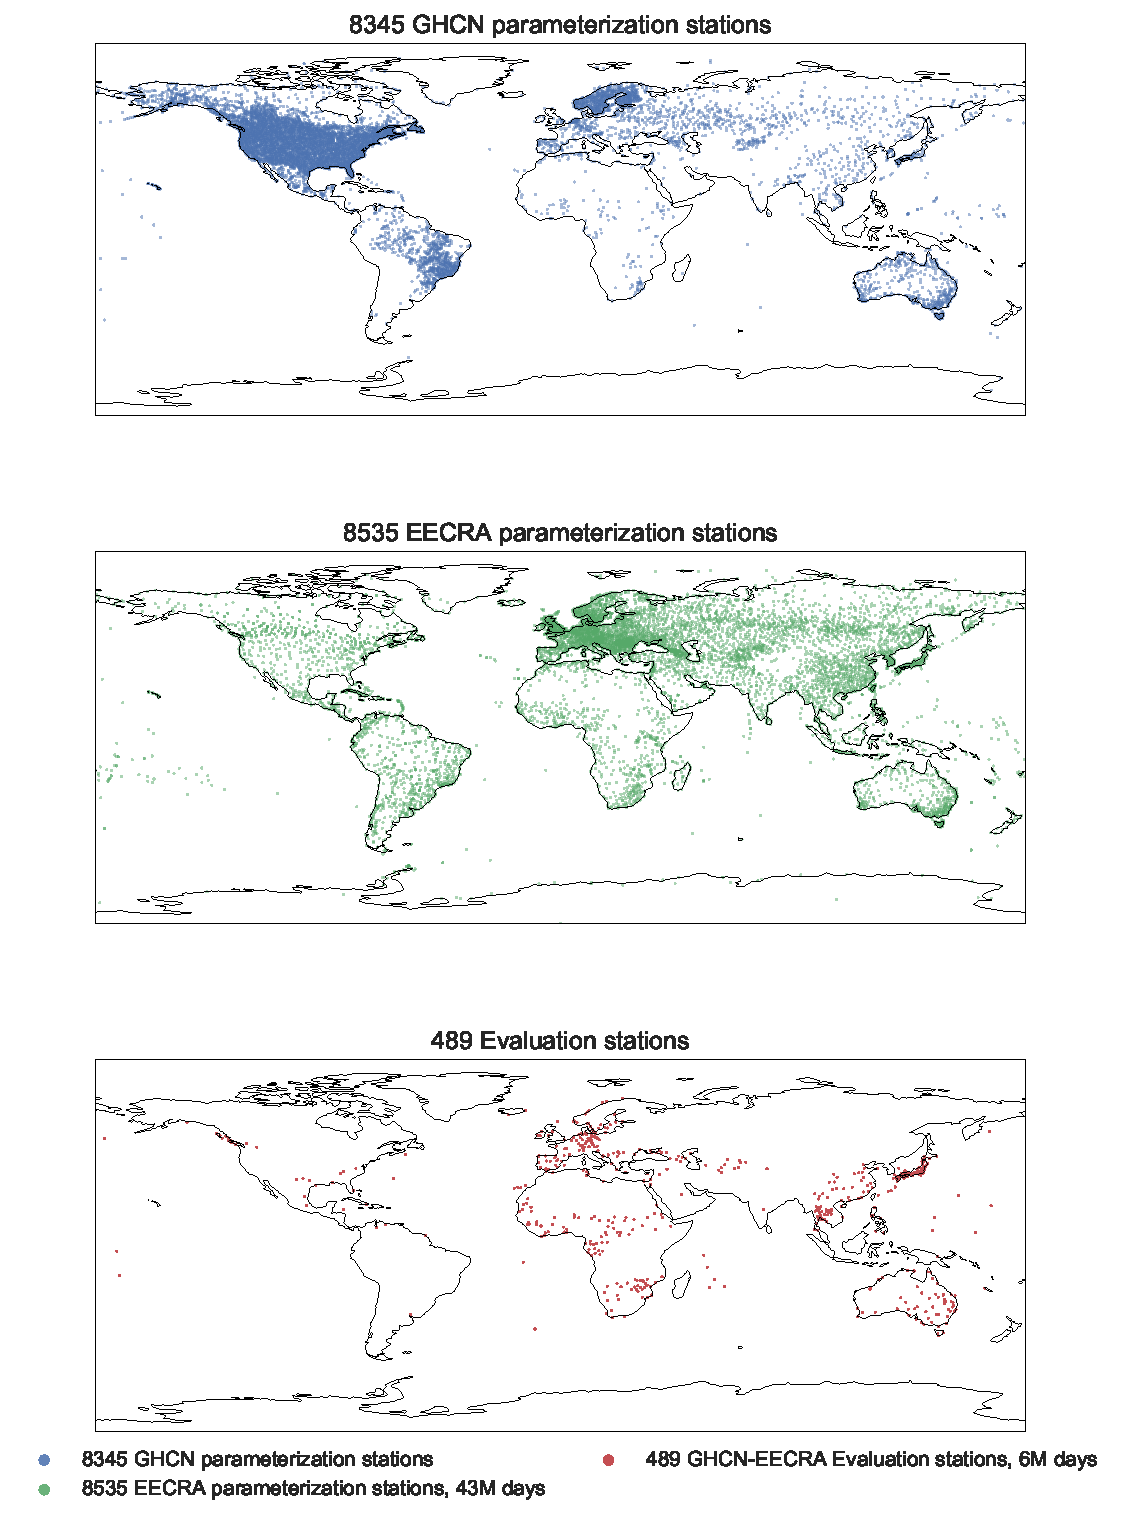
\includegraphics[width=12cm]{figures/stations_plot.pdf}
	\caption[Stations that are used for parameterization and evaluation of the weather generator.]{Stations that are used for parameterization and evaluation of the weather generator. The upper stations are used for parameterizing precipitation and temperature, the middle ones for cloud and wind parameterization, as well as the cross correlation of cloud, temperature and wind. The lower plot shows the
		evaluation stations.}
	\label{fig:stations}
\end{figure}
For the parametrization we used temperature, wind and cloud data from the Synoptic Cloud Reports (EECRA) databases \citep{HahnWarren1999}, as well as precipitation and temperature from the daily Global Historical Climatology Network (GHCN) \citep{MenneDurreVoseEtAl2012,Menne2012}. The latter consists of roughly 100'000 different stations from which we selected the one with the longest record for each grid cell in a global grid $0.5\times0.5^\circ$. Since several of the US stations measure precipitation in inches instead of millimeter per day, we furthermore selected the station that have all numbers from 0.1 to 1.0 millimeter per day in its record. This selection procedure resulted in 16'590 stations.

Our parameterization only uses months with complete records for each day of the month. The finally selected stations from the EECRA and GHCN data are displayed in figure \ref{fig:stations}.

\subsection{Parameterization} \label{sec:param}

\subsubsection{Precipitation occurrence} \label{sec:markov}

\begin{figure}
	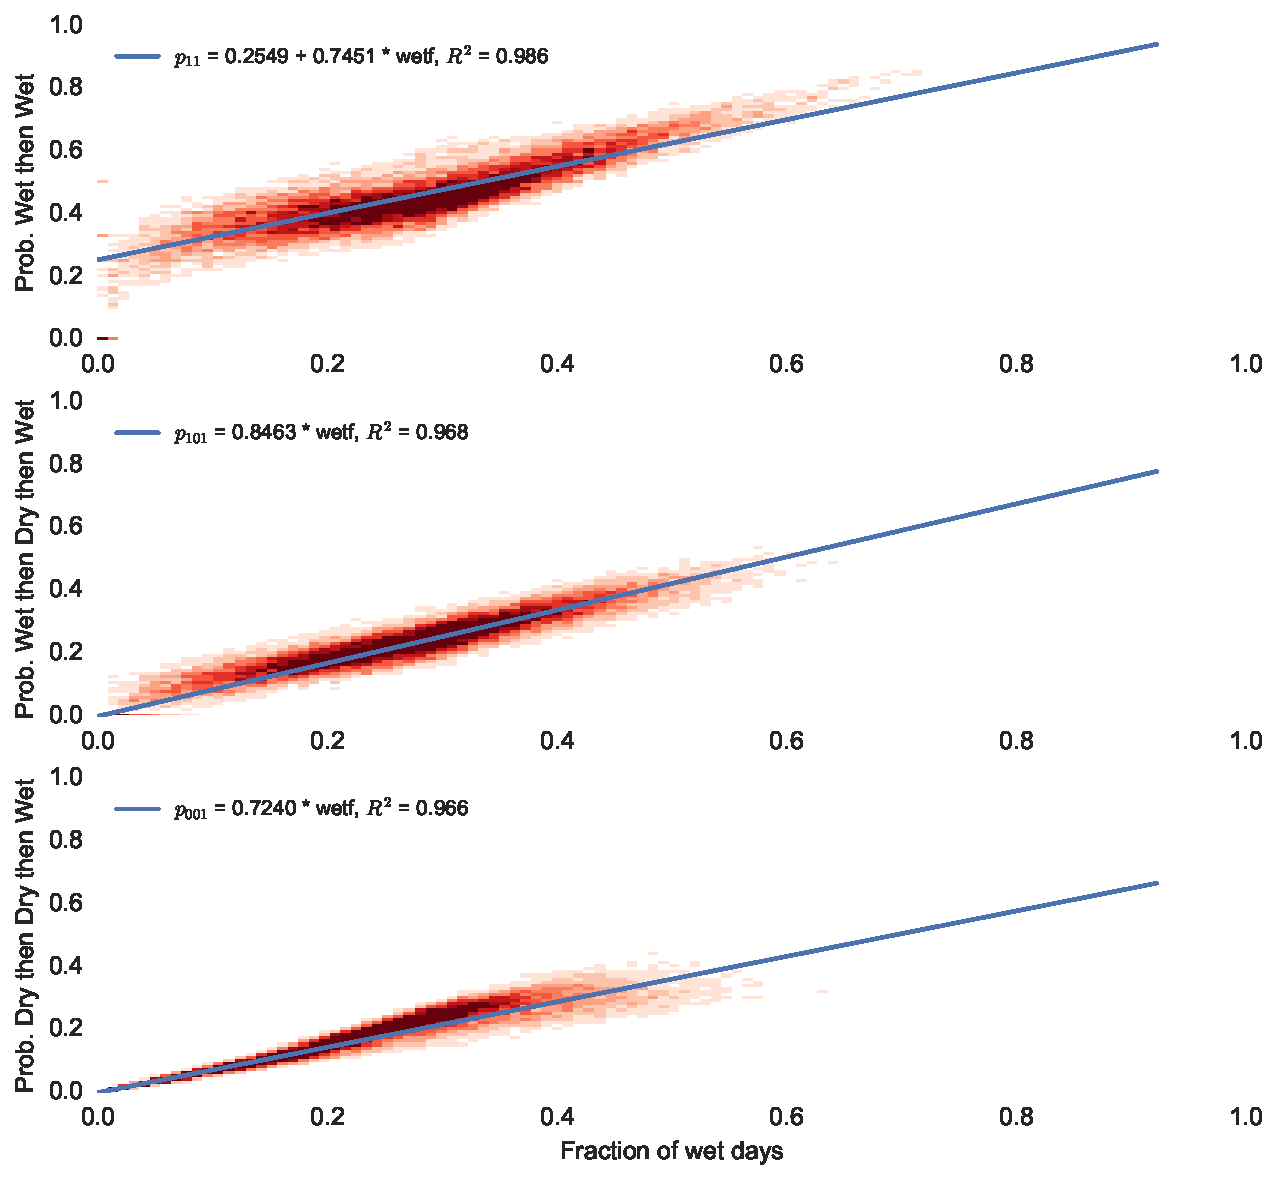
\includegraphics[width=12cm]{figures/markov.pdf}
	\caption[Transition probabilities vs. wet fraction]{Transition probabilities vs. wet fraction. The red lines show the fit of the probability against the wet fraction. The fit for the $p_{11}$ transition probability was forced to the point $(1, 1)$, the others were forced to $(0, 0)$.}
	\label{fig:markov}
\end{figure}

To apply the Markov chain, we calculated the transition probabilities for a wet day being followed by a wet day ($p_{11}$), for a wet day being followed by a dry day being followed by a wet day ($p_{101}$) and for two dry days being followed by a wet day ($p_{001})$.  We did this by first extracting all (complete) Januaries, Februaries, etc. for each of the parameterization stations separately. In a second step, all Januaries were merged together into one large multi-year series and the above mentioned transition probabilities were calculated and fitted towards the number of wet days in this series (see figure \ref{fig:markov}). Like-wise we did it for all Februaries, Marchs, etc..

%%%%%%%%%%%%%%%%% MOVE THIS TO sec:model %%%%%%%%%%%%%%%%%%%%%%%%%%%%%%
The result of this procedure are the following relationships

\begin{align}
	p_{11} &= 0.2549 + 0.7451\cdot \frac{\text{wet days in month}}{\text{days in month}} \label{eq:p11}\\
	p_{101} &= 0.8463 \cdot \frac{\text{wet days in month}}{\text{days in month}} \label{eq:p101}\\
	p_{001} &= 0.7240 \cdot \frac{\text{wet days in month}}{\text{days in month}}. \label{eq:p001}
\end{align}

Those equation are used in the weather generator to decide whether the current simulated day is a wet day or not based upon the total number of wet days in the month.
%%%%%%%%%%%%%%%%% END: MOVE THIS TO sec:model %%%%%%%%%%%%%%%%%%%%%%%%%%

\subsubsection{Precipitation amount} \label{sec:dist_params}

\begin{figure}
	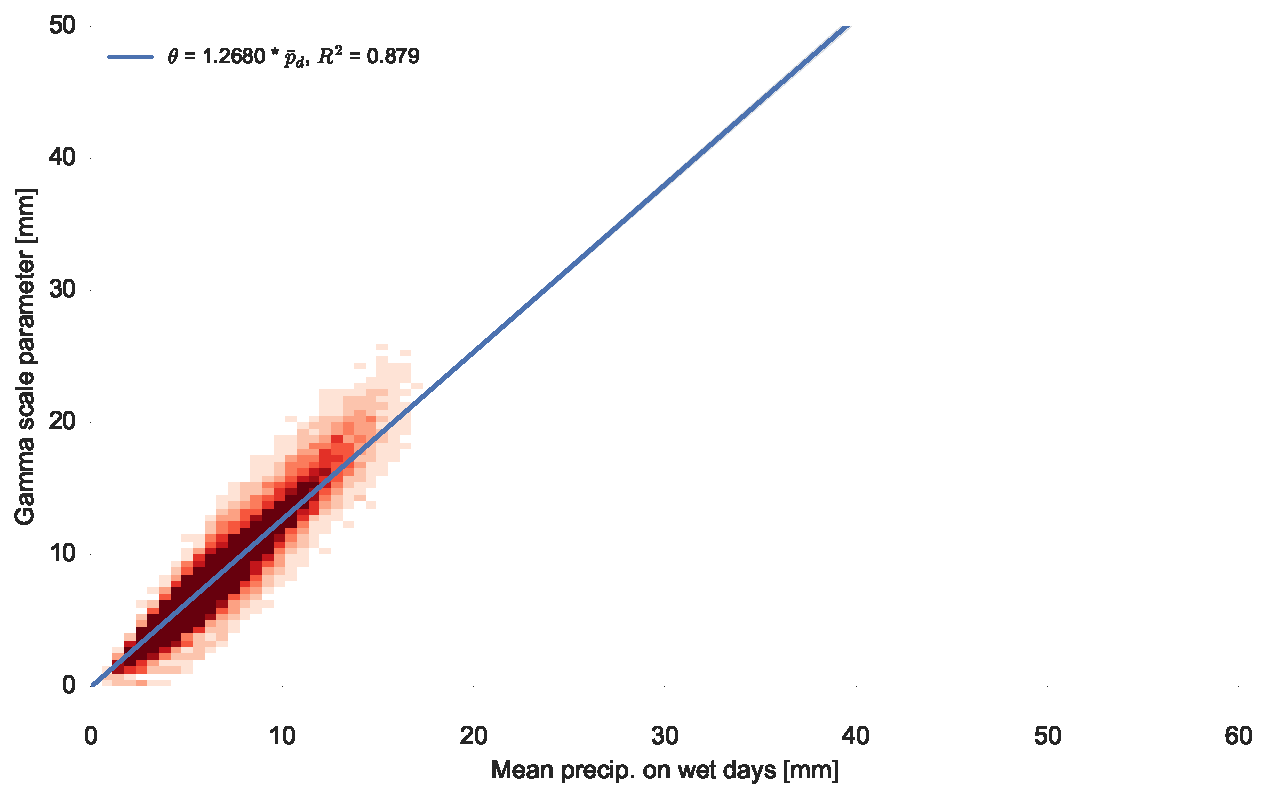
\includegraphics[width=12cm,page=1]{figures/prcp.pdf}
	\caption[Mean precipitation - Gamma scale relationship]{Mean precipitation - Gamma scale relationship. The blue line represents the best fit line of the mean precipitation on wet days to the estimated gamma scale parameter of the corresponding distribution. Each data point corresponds to one multi-year series of one month for one station.}
	\label{fig:gscale_meanw}
\end{figure}

We apply a hybrid gamma-GP distribution consisting of the the gamma and the generalized pareto (GP) distribution. The gamma distribution function is defined as
\begin{equation}
f(x) = \begin{cases}
\frac{x^{\alpha - 1}\exp^{-\frac{x}{\theta}}}{\theta^{\alpha} \Gamma(\alpha)} & \text{for } x > 0 \\
0 & \text{for } x = 0
\end{cases} \label{eq:gamma}
\end{equation}
where $\alpha > 0$ is the shape, and $\theta > 0$ the scale parameter.
The generalized pareto (GP) distribution is defined via
\begin{equation}
g(x) = \frac{1}{\sigma}\, \left( 1 + \frac{\xi\,\left(x - \mu\right)}{\sigma}\right)^{-\frac{1}{\xi} - 1} \label{eq:GP}
\end{equation}
with $\sigma > 0$ being the scale parameter and $\xi \in \mathbb{R}$ the shape parameter. $\mu$ is the location parameter.

Following \cite{FurrerKatz2008}, we define the hybrid gamma-GP distribution as
\begin{equation}
h(x) = \begin{cases}
f(x) & \text{for } x \leq \mu \\
(1 - F(\mu))\,g(x) & \text{for }  x > \mu
\end{cases}, \label{eq:GammaGP}
\end{equation}
where $F(\mu)$ describes the cumulative gamma distribution function at the threshold $\mu$. \cite{FurrerKatz2008} and \cite{NeykovNeytchevZucchini2014} have shown, that this distribution better simulates the heavy tail of the precipitation distribution than the gamma distribution alone.

To determine the parameters of the hybrid distribution for precipitation, we started with the simple stategy by \cite{GengDevriesSupit1986}. As we did above when calculating the markov chain parameters, we created multi-year series for each of the parameterization stations for each month and extracted the days with precipitation. If a series contained more than 100 entries, we fit a gamma distribution to it and estimated the $\alpha$ and $\theta$ parameters.

Following \cite{GengDevriesSupit1986}, we then fit a regression line of the gamma scale parameter against the mean precipitation on wet days $\bar{p}_d$ (see figure \ref{fig:gscale_meanw}) and found the relationship
\begin{equation}
\theta = 1.268\, \bar{p}_d. \label{eq:gamma_scale}
\end{equation}
As proposed by \cite{GengDevriesSupit1986}, we use this relationship in our model to estimate the scale parameter of the distribution. The gamma shape parameter $\alpha$ is calculated dynamically in the weather generator via
\begin{equation}
\alpha = \frac{\bar{p}_d}{\theta}. \label{eq:gamma_shape}
\end{equation}

The GP scale parameter $\sigma$ on the other hand is calculated during the simulation following \cite{NeykovNeytchevZucchini2014} via

\begin{equation}
\sigma = \frac{1 - F(\mu)}{f(\mu)}. \label{eq:gp_scale}
\end{equation}

The other parameters of the GP distribution are obtained through a sensitivity analysis described later.

\subsubsection{Temperature}

\begin{figure}
	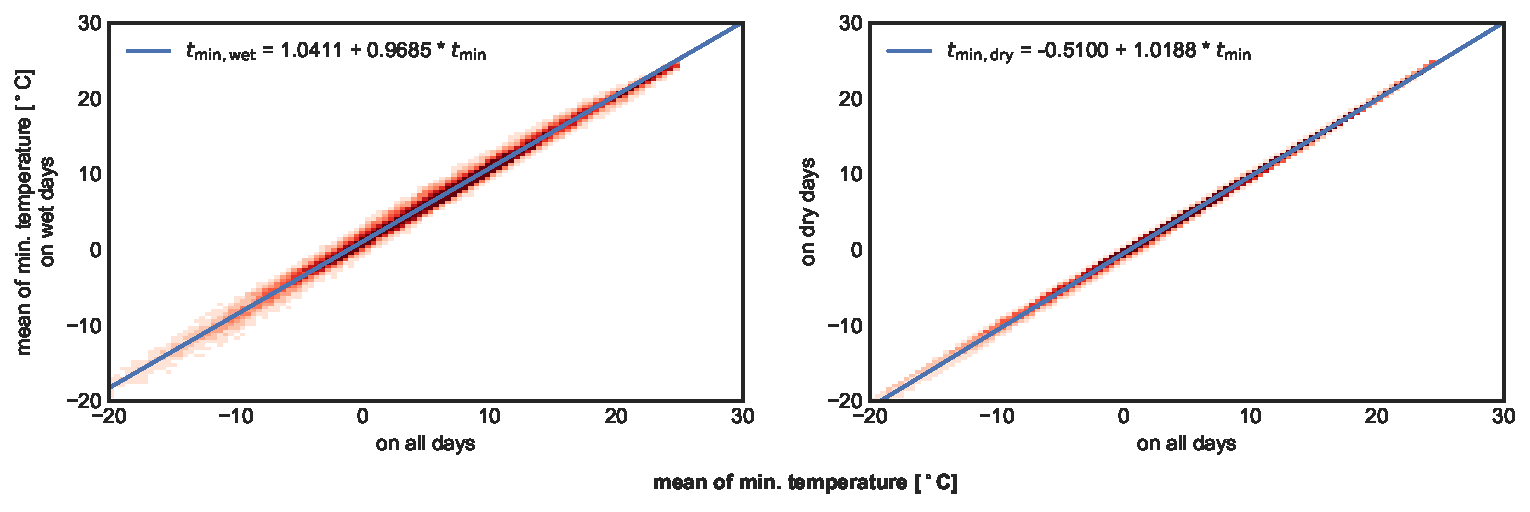
\includegraphics[width=12cm]{figures/temp.pdf}
	\caption[Correlation of minimum temperature on wet and dry days to the monthly mean]{Correlation of minimum temperature on wet and dry days to the monthly mean. The y-axes show the mean minimum temperature on wet or dry days respectively, the blue line corresponds to the best fit line. Parameters of the fits are also shown in table \ref{tab:t-corr}.}
	\label{fig:tmin}
\end{figure}
\begin{figure}
	\includegraphics[width=12cm, page=2]{figures/temp.pdf}
	\caption[Correlation of standard deviation of min. temperature to the monthly mean]{Correlation of standard deviation of the minimum temperature on wet and dry days to the monthly mean. The y-axes show the standard deviation, the x-axes the mean on wet or dry days respectively. The blue line corresponds to the best fit line. Parameters of the fits are also shown in table \ref{tab:t-corr}.}
	\label{fig:tmin_sd}
\end{figure}
\begin{figure}
	\includegraphics[width=12cm, page=3]{figures/temp.pdf}
	\caption[Correlation of maximum temperature on wet and dry days to the monthly mean]{Correlation of maximum temperature on wet and dry days to the monthly mean. The y-axes show the mean maximum temperature on wet or dry days respectively, the blue line corresponds to the best fit line. Parameters of the fits are also shown in table \ref{tab:t-corr}.}
	\label{fig:tmax}
\end{figure}
\begin{figure}
	\includegraphics[width=12cm, page=4]{figures/temp.pdf}
	\caption[Correlation of standard deviation of min. temperature to the monthly mean]{Correlation of standard deviation of the minimum temperature on wet and dry days to the monthly mean. The y-axes show the standard deviation, the x-axes the mean on wet or dry days respectively. The blue line corresponds to the best fit line. Parameters of the fits are also shown in table \ref{tab:t-corr}.}
	\label{fig:tmax_sd}
\end{figure}
\begin{table}[t]
	\caption[Fit results of temperature correlation for wet and dry days.]{Fit results of temperature correlation for wet and dry days for figure \ref{fig:tmin} and \ref{fig:tmax}. $N$ is the total number of measurements used for the fit. The values of $a$ and $b$ correspond to the values in equation \eqref{eq:linear} and \eqref{eq:sd_linear}.}
	\label{tab:t-corr}
	\begin{tabular}{llccccc}
\tophline
              plot &                          variable &  $R^2$ &   $c_0$ &  $c_1$ &   $c_2$ &  $c_3$ \\
\middlehline
 \ref{fig:tmax} &  $T_{\mathrm{max}, \mathrm{dry}}$ & 0.9969 & 0.0727 & 1.0211 & 0 & 0 \\
 \ref{fig:tmax} &  $T_{\mathrm{max}, \mathrm{wet}}$ & 0.9752 & -0.5204 & 0.9459 & 0 & 0 \\
 \ref{fig:tmin} &  $T_{\mathrm{min}, \mathrm{dry}}$ & 0.9972 & -0.5100 & 1.0188 & 0 & 0 \\
 \ref{fig:tmin} &  $T_{\mathrm{min}, \mathrm{wet}}$ & 0.9840 & 1.0411 & 0.9685 & 0 & 0 \\
 \ref{fig:wind_sd} &  $w_{\mathrm{sd}, \mathrm{dry}}$ & 0.4243 & 0 & 1.0860 & -0.2407 & 0.0222 \\
 \ref{fig:wind_sd} &  $w_{\mathrm{sd}, \mathrm{wet}}$ & 0.5003 & 0 & 0.8184 & -0.1263 & 0.0093 \\
 \ref{fig:wind} &  $w_{\mathrm{dry}}$ & 0.9930 & 0 & 0.9437 & 0 & 0 \\
 \ref{fig:wind} &  $w_{\mathrm{wet}}$ & 0.9723 & 0 & 1.0937 & 0 & 0 \\
\bottomhline
\end{tabular}

\end{table}

For each day we know from the Markov chain approach, whether the current simulated day is a wet or dry day. Based upon the simple linear relationships

\begin{align}
	x_\mathrm{wet} &= a_{x, \mathrm{wet}} + b_{x, \mathrm{wet}} \cdot \bar{x} \nonumber \\
	x_\mathrm{dry} &= a_{x, \mathrm{dry}} + b_{x, \mathrm{dry}} \cdot \bar{x} \label{eq:linear}
\end{align}

we adjust the monthly mean $\bar{x}$ of the variable $x\in\{T_\mathrm{min}, T_\mathrm{max}\}$. The intercept $a$ and slope $b$ of those linear relationships have been determined through a fit of the mean maximum and minimum temperature on wet or dry days in one month to the overall monthly mean (see figures \ref{fig:tmin}, \ref{fig:tmax} and table \ref{tab:t-corr}) on our parameterization data.

The standard deviation  $\sigma_x$ of variable $x\in\{T_\mathrm{min}, T_\mathrm{max}\}$ is then calculated from the adjusted mean via

\begin{align}
	\sigma_{x, \mathrm{wet}} &= a_{\sigma, x, \mathrm{wet}} + b_{\sigma, x, \mathrm{wet}} \cdot x_\mathrm{wet} \nonumber \\
	\sigma_{x, \mathrm{dry}} &= a_{\sigma, x, \mathrm{dry}} + b_{\sigma, x, \mathrm{dry}} \cdot x_\mathrm{dry}. \label{eq:sd_linear}
\end{align}

To estimate the values of the parameters $a$ and $b$ in equation \eqref{eq:sd_linear}, we used a fit to the GHCN data (figures \ref{fig:tmin_sd}, \ref{fig:tmax_sd} and table \ref{tab:t-corr}). The linear model does not really satisfy  the complex behaviour of the standard deviation, but since this value is only used for the random noise (see below), we think that the error is negligible.

\subsubsection{Cloud fraction}
\begin{figure}
	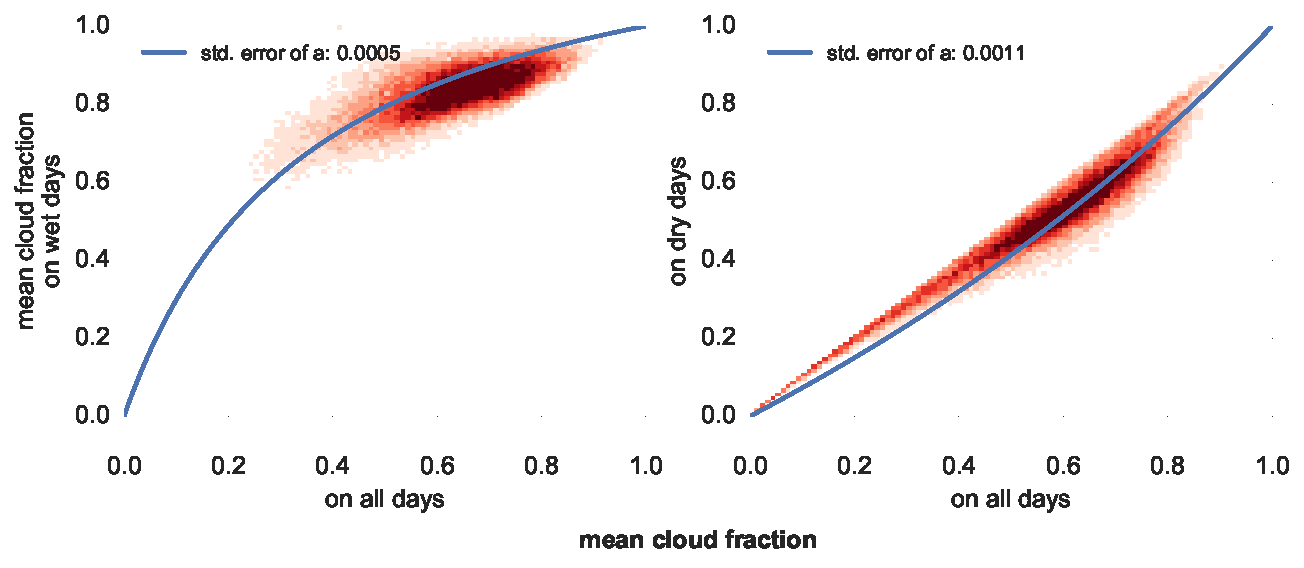
\includegraphics[width=12cm]{figures/cloud.pdf}
	\caption[Correlation of cloud fraction on wet and dry days to the monthly mean]{Correlation of cloud fraction on wet and dry days to the monthly mean.The y-axes show the mean cloud fraction on wet or dry days respectively, the blue line corresponds to the best fit line. Parameters of the fits are also shown in table \ref{tab:cloud-corr}.}
	\label{fig:cloud}
\end{figure}
\begin{figure}
	\includegraphics[width=12cm, page=2]{figures/cloud.pdf}
	\caption[Correlation of standard deviation of cloud fraction to the monthly mean]{Correlation of standard deviation of the cloud fraction on wet and dry days to the corresponding monthly mean. The y-axes show the standard deviation, the x-axes the mean on wet or dry days respectively. The blue line corresponds to the best fit line. Parameters of the fits are also shown in table \ref{tab:cloud-corr}.}
	\label{fig:cloud_sd}
\end{figure}
\begin{table}[t]
	\caption[Fit results of cloud correlation for wet and dry days.]{Fit results of cloud correlation for wet and dry days for figure \ref{fig:cloud}}
	\label{tab:cloud-corr}
	\begin{tabular}{llcc}
\tophline
               plot &                         variable &       a & std. dev. of a \\
\middlehline
 \ref{fig:cloud} &  $c_{\mathrm{dry}}$ & 0.4205 & 0.0011 \\
 \ref{fig:cloud} &  $c_{\mathrm{wet}}$ & -0.7383 & 0.0005 \\
 \ref{fig:cloud_sd} &  $c_{\mathrm{sd}, \mathrm{dry}}$ & 1.0417 & 0.0003 \\
 \ref{fig:cloud_sd} &  $c_{\mathrm{sd}, \mathrm{wet}}$ & 0.9819 & 0.0005 \\
\bottomhline
\end{tabular}

\end{table}

To parameterize the cloud fraction, we first calculated the variable from the EECRA dataset. The original dataset contains eight measurements per day of the total cloud cover ranging from 0 (clear sky) to 8 (overcast). Hence, to calculate the daily cloud fraction, those values were averaged and divided by 8 to get the daily mean.

To adjust the monthly mean depending on the wet-dry state of the day, we could not use the simple linear relationship as we used for temperature because the cloud fraction bounded by the lower limit 0 and the upper limit 1. However, the cloud cover on wet days is usually greater or equal to the monthly mean cloud cover whereas the cloud cover on dry days is usually less or equal to the monthly mean cloud cover. This results in a concave curve for the wet case and a convex curve for dry days. Therefore we came up with the following formula for the fit:

\begin{align}
	\mathrm{c}_\mathrm{wet} &= \frac{-a_{\mathrm{c}, \mathrm{wet}} - 1}{a_{\mathrm{c}, \mathrm{wet}}^2 * c - a_{\mathrm{c}, \mathrm{wet}}^2 - a_{\mathrm{c}, \mathrm{wet}}}  - \frac{1}{a_{\mathrm{c}, \mathrm{wet}}} \nonumber \\
	\mathrm{c}_\mathrm{dry} &= \frac{-a_{\mathrm{c}, \mathrm{dry}} - 1}{a_{\mathrm{c}, \mathrm{dry}}^2 * c - a_{\mathrm{c}, \mathrm{dry}}^2 - a_{\mathrm{c}, \mathrm{dry}}}  - \frac{1}{a_{\mathrm{c}, \mathrm{dry}}}
	\label{eq:cloud_mean}
\end{align}

with $a_{\mathrm{c}, \mathrm{wet}} < 0$ and $a_{\mathrm{c}, \mathrm{dry}} > 0$.

The standard deviation on the other hand becomes 0 when the amount of mean monthly cloud fraction reaches the outer limits 0 and 1. Hence we have an concave parabola with the formula

\begin{align}
	\sigma_{\mathrm{c}, \mathrm{wet}} &= a_{\mathrm{c}, \mathrm{wet}}^2 \cdot \mathrm{c}_\mathrm{wet} \cdot (1 - \mathrm{c}_\mathrm{wet}) \nonumber \\
	\sigma_{\mathrm{c}, \mathrm{dry}} &= a_{\mathrm{c}, \mathrm{dry}}^2 \cdot \mathrm{c}_\mathrm{dry} \cdot (1 - \mathrm{c}_\mathrm{dry}) \label{eq:cloud_sd}
\end{align}

with $a_{\mathrm{c}, \mathrm{wet}}, a_{\mathrm{c}, \mathrm{dry}} \geq 0$. Results of the fits can be seen in figure \ref{fig:cloud}, \ref{fig:cloud_sd} and table \ref{tab:cloud-corr}.


\subsubsection{Wind speed}
\begin{figure}
	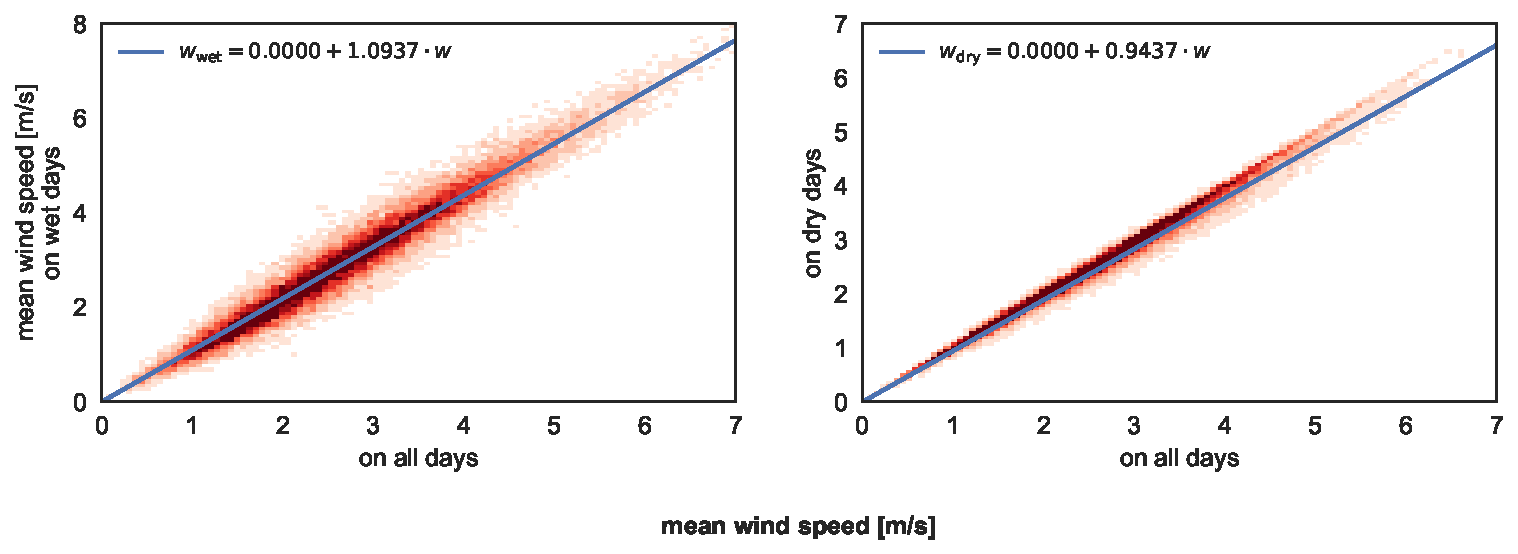
\includegraphics[width=12cm]{figures/wind.pdf}
	\caption[Correlation of wind speed on wet and dry days to the monthly mean]{Correlation of wind speed on wet and dry days to the monthly mean.The y-axes show the mean cloud fraction on wet or dry days respectively, the blue line corresponds to the best fit line. Parameters of the fits are also shown in table \ref{tab:t-corr}.}
	\label{fig:wind}
\end{figure}
\begin{figure}
	\includegraphics[width=12cm, page=2]{figures/wind.pdf}
	\caption[Correlation of standard deviation of wind speed to the monthly mean]{Correlation of standard deviation of the wind speed on wet and dry days to the corresponding monthly mean. The y-axes show the standard deviation, the x-axes the mean on wet or dry days respectively. The blue line corresponds to the best fit line. Parameters of the fits are also shown in table \ref{tab:t-corr}.}
	\label{fig:wind_sd}
\end{figure}

The parameterization of wind speed is based upon the same equations \eqref{eq:linear} and \eqref{eq:sd_linear} as temperature and shown in the figures \ref{fig:wind} and \ref{fig:wind_sd}. Following \cite{ParlangeKatz2000} we additionally use a square root transformation (see line \ref{a:gwgen:cross-end} in the model algorithm \ref{a:gwgen}). 


\subsubsection{Cross correlation} \label{sec:corr}
Following \cite{Richardson1981} we use cross correlation to calculate the residuals and, following \cite{ParlangeKatz2000}, we use a square root transformation for the wind speed.

From the data in the EECRA database for the cloud parameterization (see figure \ref{fig:stations}) we get the
\begin{equation}
A = \begin{matrix}
  0.916 & 0.031 & -0.018 & 0.001\\
  0.485 & 0.135 & -0.069 & -0.047\\
  0.004 & -0.043 & 0.592 & 0.023\\
  0.012 & -0.043 & -0.02 & 0.672\\
\end{matrix}
\qquad
B = \begin{pmatrix}
  0.362 & 0. & 0. & 0.\\
  0.114 & 0.803 & 0. & 0.\\
  0.145 & -0.061 & 0.783 & 0.\\
  0.081 & -0.016 & 0.066 & 0.737\\
\end{pmatrix} \label{eq:AB}
\end{equation}

where the columns and rows correspond to min. and max. temperature, cloud fraction and square root of wind speed.

The above matrices \eqref{eq:AB} where calculated via

\begin{equation}
A = M_1M_0^{-1} \qquad BB^T = M_0 - M_1M_0^{-1}M_1^T
\end{equation}

from the lag-0 and lag-1 covariance  matrices $M_0$ and $M_1$ with

\begin{equation}
M_0 = \begin{matrix}
  1. & 0.565 & 0.041 & 0.035\\
  0.565 & 1. & -0.089 & -0.043\\
  0.041 & -0.089 & 1. & 0.114\\
  0.035 & -0.043 & 0.114 & 1.\\
\end{matrix}
\qquad
M_1 = \begin{pmatrix}
  0.932 & 0.557 & -0.001 & 0.025\\
  0.564 & 0.426 & -0.08 & -0.046\\
  -0.012 & -0.108 & 0.6 & 0.104\\
  0.006 & -0.066 & 0.071 & 0.667\\
\end{pmatrix}.
\end{equation}

\subsection{Evaluation} \label{sec:eval}
\begin{figure}
	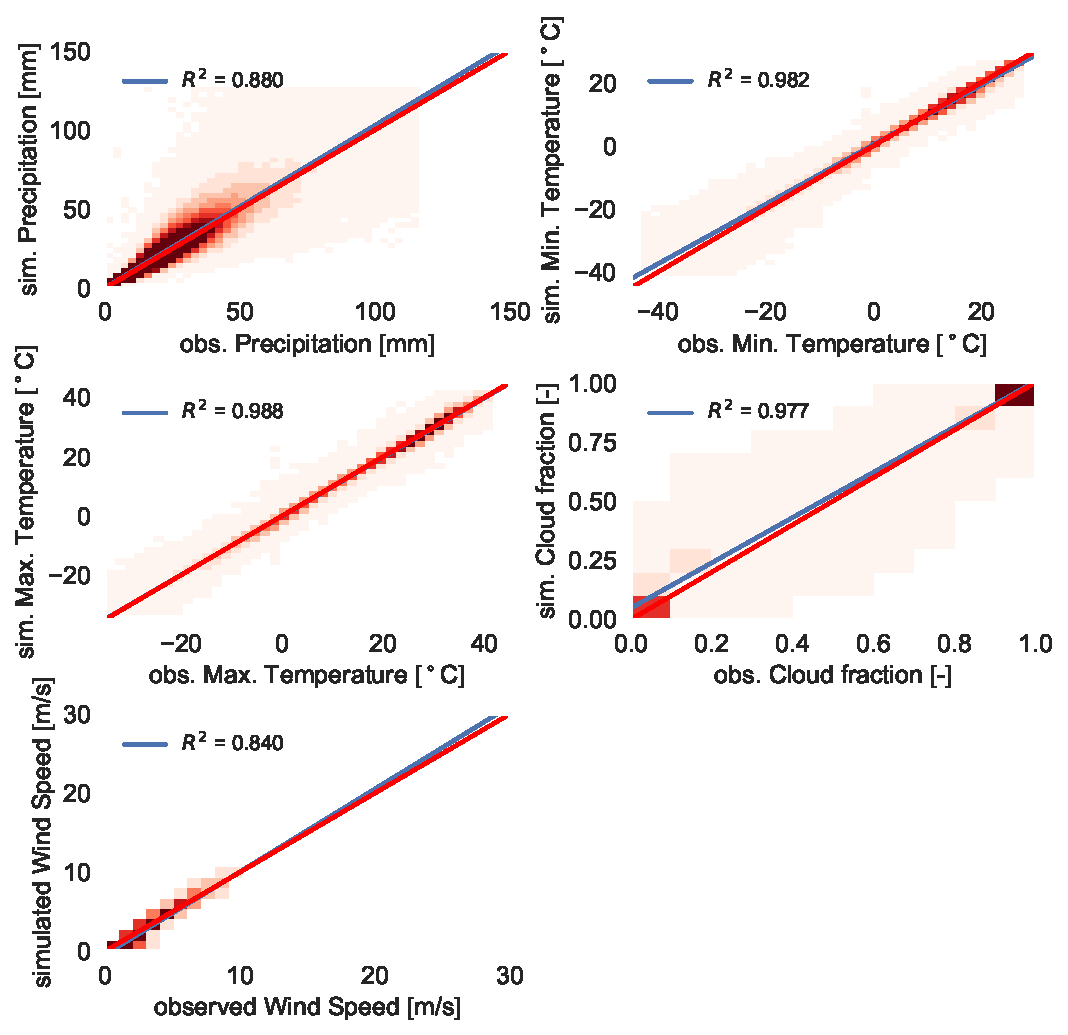
\includegraphics[width=12cm, page=1]{figures/quants.pdf}
	\caption[QQ-plots for all variables and all quantiles]{QQ-plots for all variables with all quantiles (1, 5, 10, 25, 50, 75, 90, 95 and 99) for ${\mu=\ldots\, \mathrm{mm}}$, $\xi=\ldots$. The blue lines are linear regression from simulation to observation. The red line shows the ideal fit (the identity line). Blue shaded areas represent the $95\%$ confidence interval. Plots for wind speed and minimum temperature used the bias correction from \autoref{sec:bias}.}
	\label{fig:all_quants}
\end{figure}
\begin{figure}
	\includegraphics[width=12cm, page=3]{figures/quants.pdf}
	\caption[QQ-plots for different quantiles for precipitation]{QQ-plot for different quantiles for precipitation for ${\mu=15\, \mathrm{mm}}$, $\xi=0.08303$. The blue lines are linear regression from simulation to observation. The red line shows the ideal fit (the identity line). Blue shaded areas represent the $95\%$ confidence interval.}
	\label{fig:precip_quants}
\end{figure}
%Furthermore we merged the data from the cloud database into the GHCN dataset. In the first step we found all GHCN stations that are within a radius of one kilometer for each station in the EECRA database. In the second step we then merged the EECRA station into the GHCN dataset based upon the closest station found (if existent). This procedure resulted in about 3'400 stations from the cloud database that could be merged into the GHCN dataset.
%
%For validation purposes, we took 500 stations out of the 16'590 mentioned above, excluded them from the parameterization and used them for evaluation. Our parameterization then also only uses months with a complete record and the evaluation uses only yearly complete series. The finally used stations are shown in figure \ref{fig:stations}.

To evaluate our model, we merged the EECRA dataset into the GHCN data. For each station in the EECRA database we identified the closest GHCN station within 1km. Doing so, resulted in about 1200 stations. We compared the simulated years against the observed years and hence took only the complete years per station. This resulted in about 500 evaluation stations, shown in figure \ref{fig:stations}.

We calculated the monthly input for our weather generator and compared the daily simulation from our model to the original daily data. Since we cannot expect from the weather generator to represent the exact timing during the month, we are restricted to compare the two distributions.

Figure \ref{fig:all_quants} shows the comparison of the simulated versus the observed quantiles. For temperature, wind and cloud fraction, the model does an excellent job of downscaling monthly input to daily resolution. Also precipitation looks good when mangling all the quantiles, however, a closer look into figure \ref{fig:precip_quants} shows that the higher precipitation percentiles are well captured using the hybrid Gamma-GP distribution, the lower percentiles however show worse results. The same holds for the wind speed (not shown here). The lower values of the two variables, however, are very close to the precision of the observation ($0.1\, \unit{mm}$ for precipitation and $0.1\, \unit{m/s}$ for wind speed). Secondly, they are ecologically not as important as the higher percentiles.\footnote{Note that the plots for wind speed and minimum temperature were bias corrected using the approach in \autoref{sec:bias}.}

In table \ref{tab:freq} we also compare the simulated versus the observed frequencies. For very light rain (<=1mm), light rain (1-10mm), heavy rain (10-20mm) and very heavy rain (>20mm). As we can see, our model underestimates the occurence of very light rain events ($21.6\%$ instead of $27.0\%$) and overestimates the light rain events ($55\%$ instead of $47\%$) but performs much better than other climate models \citep{Dai2006,SunSolomonDaiEtAl2006}, especially when it comes to the heavy rain events.

\begin{table}
	\caption[Simulated and observed precipitation frequencies.]{Simulated and observed precipitation frequencies for certain ranges. The frequency is defined as the number of precipitation occurences in the specified range, divided by the total number of precipitation occurences.}
	\label{tab:freq}
	\begin{tabular}{lrr}
		\tophline
		{} &  Simulated &  Observed \\
		Precipitation [mm]      &            &           \\
		\middlehline
		(0, 1]    &      0.216 &     0.270 \\
		(1, 10]   &      0.550 &     0.470 \\
		(10, 20]  &      0.115 &     0.133 \\
		(20, $\infty$) &      0.120 &     0.127 \\
		\bottomhline
	\end{tabular}
\end{table}


\subsection{Bias correction} \label{sec:bias}
\begin{figure}
	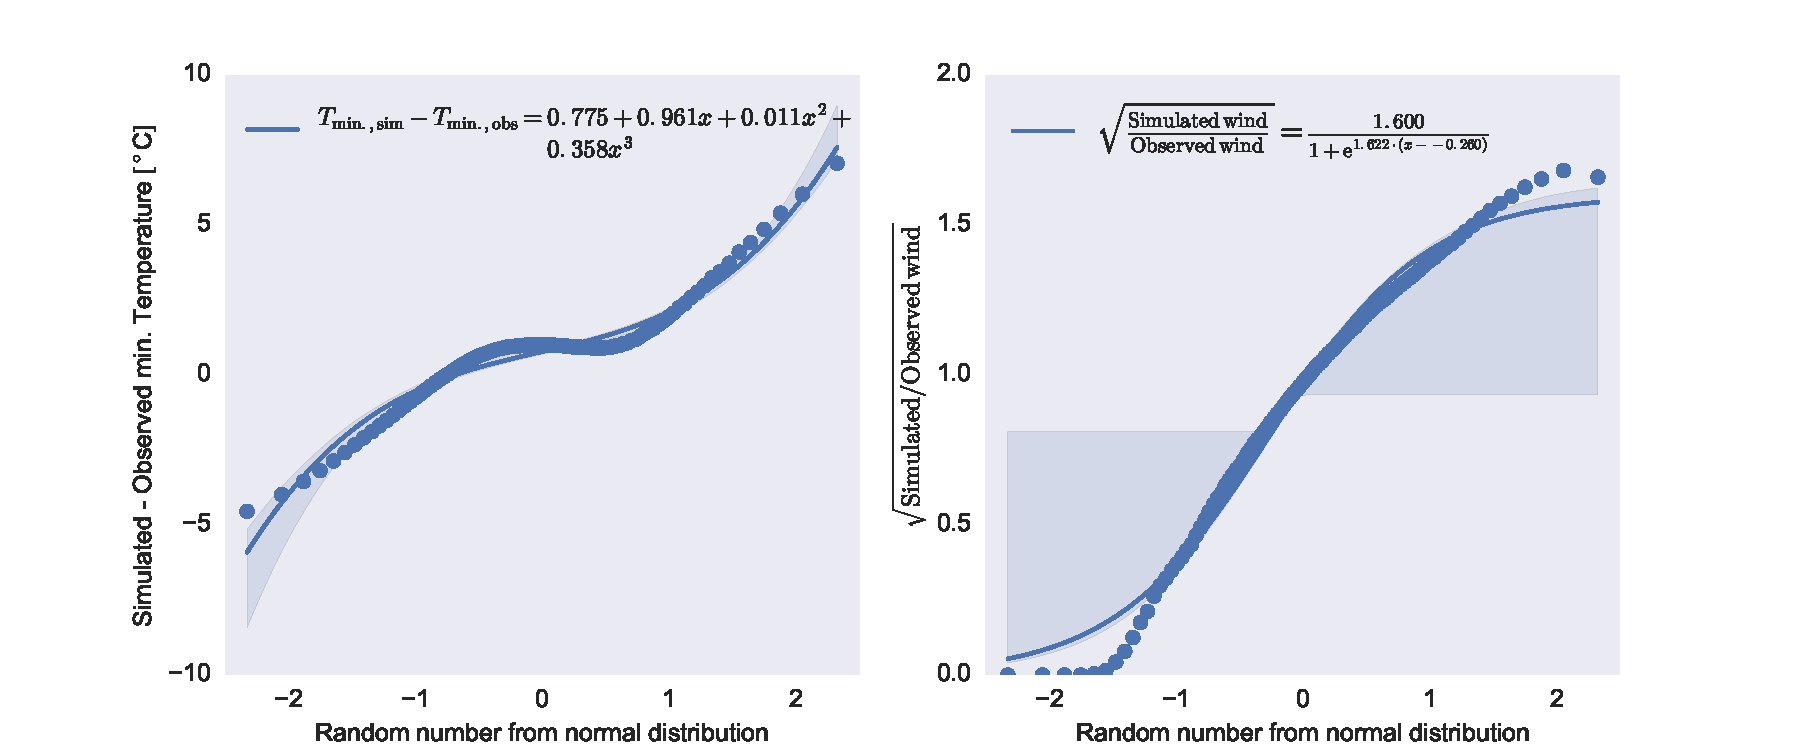
\includegraphics[width=12cm]{figures/wind_tmin_bias_correction.pdf}
	\caption[min. temperature and wind bias correction]{Basis for the minimum temperature (left) and wind bias correction (right). For the left plot (min. Temperature), each data point corresponds to the difference of a simulated percentile to the observed percentile. For the right plot (wind speed), each data point corresponds to the fraction of simulated to the observed square root of the wind speed for a given percentile. The random number on the x-axis represents the residual value from a normal distribution centered at 0 with standard deviation of unity, as it is used in the cross correlation approach \citep{Richardson1981}.}
	\label{fig:bias}
\end{figure}

After evaluating the results of GWGEN for wind speed and minimum temperature for the different quantiles (see previous \autoref{sec:eval}) we found a strong correlation between the deviation from the simulated and the observed quantile.

For the minimum temperature, we use an empirical distribution correction approach (quantile-mapping, \cite{LafonDadsonBuysEtAl2012}) with the third order polynomial shown in figure \ref{fig:bias} to transform the simulated minimum temperature data based upon the modeled quantile. The coefficients of this polynomial are calculated a posteriori based upon the bias from simulated to the observed quantile for all percentiles between 1 and 99. The resulting function $f_{T_\mathrm{min}}(u)$ is then used in the weather generator to correct the minimum temperature $T_\mathrm{min}$ via
\begin{equation}
T_\mathrm{min} = T_{\mathrm{min}, biased} - f_{T_\mathrm{min}}(u) \label{eq:bias-tmin}
\end{equation}
where $u\in\mathbb R$ corresponds to the number from the normal distribution drawn for the cross correlation (section \ref{sec:corr} and \cite{Richardson1981}).

Furthermore, we found that the fraction of simulated to observed wind speed for a given percentile follows strongly a logistic function or a third order polynomial (figure \ref{fig:bias}). Hence, as we did for minimum temperature, we use a quantile mapping approach and a posteriori correlate the square root of the fraction of simulated to observed wind speed with the percentile in the normal distribution. The resulting function $f(u)$, is then used inside the weather generator to correct the the wind speed $w$ via
\begin{equation}
w = w_\mathrm{biased} \ f(u). \label{eq:bias-wind}
\end{equation}.


\subsection{Sensitivity analysis}
Our hybrid Gamma-GP distribution has two parameters, the GP shape and the threshold parameter, which could not be related in a sufficiently sophisticated way to any of the simulated variables. Hence, we determined the parameters using a sensitivity analysis.

We chose two methods: the first one is the direct comparison of the quantiles (see previous section), the second one is a Kolmogorov-Smirnov (KS) test that evaluates whether two data samples come from significantly different distributions. Our criteria where

\begin{enumerate}
	\item The $R^2$  correlation coefficient between simulated and observed quantiles \label{item:sens_rsquared}
	\item The fraction $\frac{\text{simulated precipitation}}{{\text{observed precipitation}}}$ from the slopes in \ref{fig:precip_quants} and it's deviation from unity \label{item:sens_slope}
	\item the fraction of simulated (station specific) years that are significantly different from the observation \label{item:sens_ks}
	\item The mean of the above values \label{item:sens_mean}
\end{enumerate}

We tried two different approaches for the threshold: firstly, a fixed crossover point, secondly a quantile based crossover point. For the latter, the model chooses to use the GP distribution if the quantile of the drawn random number is above a certain  quantile. This introduces a flexible crossover point in our hybrid distribution which, however, did not improve the results significantly. Hence we decided to only show the results of the fixed crossover point.

The values of the crossover point for  our sensitivity analysis were 2, 2.5, 3, 4 and from 5 to 100 in steps of 5. Furthermore we varied the GP shape parameter from 0 to 3 in steps of 0.1 (810 experiments in total). The results of this sensitivity analysis are shown in the supplementary material, figure \ref{fig:sens}.

In general we found that the three criteria \ref{item:sens_rsquared}, \ref{item:sens_slope} and \ref{item:sens_ks} could not be optimized all together at the same time. The $R^2$ is best for high thresholds and low GP shape parameters, the slope is best for intermediate threshold and a high GP shape and the KS statistic is best for low threshold and intermediate GP shape parameters.

However, $R^2$ did not vary that much (from 0.68 to 0.74) and from a visual evaluation of the corresponding quantile plots we saw that the higher quantiles (>90) were much better represented for a better KS result. Hence we chose to follow the KS test criteria, which is also the strictest of our evaluation methods but again compared the different quantile plots to get good results for the higher quantiles.  Finally, we chose a threshold of $5\,\unit{mm}$ and a GP shape parameter of $1.5$. For this setting, $83.6\%$ of the simulated years do not show a significant difference compared to the observation, the mean $R^2$ of the plots in figure \ref{fig:precip_quants} is $0.70$ and the mean deviation of the slope from unity is $0.18$ and for the upper quantiles (90 to 100), $0.1$.

Nevertheless, in total the results seem to be fairly independent of the two parameters since even the amount of years without significant differences vary from $70\%$ to only $86\%$. It is however better than the gamma distribution alone with only $76.2\%$ of station years not differing significantly and a slope deviation from unity for the upper quantiles of $0.26$.


\section{Model description} \label{sec:model}
The parameterization described in section \ref{sec:param} is incorporated into a stand-alone model. It requires additional total monthly precipitation, the number of wet days, mean minimum and maximum temperature, mean cloud fraction and wind speed as input. The output are the same variables with daily resolution. This section summarizes the basic workflow in the model which is also shown schematically in algorithm \ref{a:gwgen}.

The first approximation of the daily variables comes from smoothing the monthly time series using the algorithm described in \cite{RymesMyers2001}.

For precipitation we then first use the markov chain approach from section \ref{sec:markov} to decide the wet/dry state of the day. If the day is a wet day, we calculate the gamma parameters using the equations \eqref{eq:gamma_scale} and \eqref{eq:gamma_shape}. The resulting distribution allows us to draw a random number, the precipitation amount of the currently simulated day. If we are above the threshold $\mu$, we draw a second random number from the GP distribution parameterized via equation \eqref{eq:gp_scale} and the chosen GP shape.

The next step modifies the means of temperature, wind speed and cloud fraction depending on the wet/dry state of the day (lines \ref{a:gwgen:adjust_wet} and \ref{a:gwgen:adjust_dry} in algorithm \ref{a:gwgen}). After that, we use the cross-correlation approach described in \cite{Richardson1981} and lines \ref{a:gwgen:cross} - \ref{a:gwgen:cross-end} and calculate the other variables. Finally we use the quantile-based bias correction described in section \ref{sec:bias} to correct the simulated wind speed and minimum temperature.

We restrict the weather generator to reproduce the exact number of wet days ($\pm1$) as the input and to be within a $5\%$ range of the total monthly precipitation (with a maximum allowed deviation of $0.5\,\unit{mm}$). Hence, if the program cannot produce these results, the procedure described above is repeated (see line \ref{a:gwgen:accuracy-criteria}).

\begin{algorithm}
	\renewcommand{\algorithmicensure}{\textbf{Output:}}
	\caption{Basic workflow of GWGEN}
	\label{a:gwgen}
	\begin{algorithmic}[1]
		\REQUIRE monthly precipitation $P_\mathrm{in}\, [\unit{mm}]$, cloud cover fraction $c_\mathrm{in}$, minimum ( $T_{\mathrm{min}, \mathrm{in}}\, [^\circ\unit{C}]$) and maximum ( $T_{\mathrm{max}, \mathrm{in}}\, [^\circ\unit{C}]$) temperature, wind speed $w_\mathrm{in}\, [\unit{m/s}]$, number of wet days $n_\mathrm{in}$
		\ENSURE daily $P_i\, [\unit{mm/d}], c_i, T_i\, [^\circ\unit{C}], w_i \, [\unit{m/s}]$ and the wet/dry state $s_i\in\{0, 1\}$
		\FOR{month $m$ in $input$}
		\STATE smooth the monthly data using \cite{RymesMyers2001}
		%		\WHILE{the total simulated precipitation deviates more than $5\%$ or $0.5\,\unit{mm}$ from $P_\mathrm{in}$, or the number of simulated wet days deviates more than one from $n_\mathrm{in}$} \label{a:gwgen:accuracy-criteria}
		\WHILE{$\left|\sum_{d_i \in m} P_i - P_\mathrm{in}\right| > \mathrm{min}\left(5\%\cdot P_\mathrm{in}, 0.5mm\right)$ or $\left|n_\mathrm{sim} - n_\mathrm{in}\right| > 2$} \label{a:gwgen:accuracy-criteria}
		\FOR{day $d_i$ in $m$}
		\STATE Calculate $p_{11}, p_{101}, p_{001}$ after equations \eqref{eq:p11} - \eqref{eq:p001} using $n$ 				\COMMENT{Precipitation occurence after \cite{Wilks1999}}
		\STATE Use the Markov chain to determine whether $d_i$ is wet ($s_i = 1$) or dry ($s_i = 0$)
		%				\STATE Draw a random number $u\in[0, 1]$
		%				\IF{$P_{i-1} > 0$}
		%					\STATE $d_i$ is wet if and only if $u>p_{11}$
		%				\ELSIF{$P_{i-2} > 0$}
		%				   \STATE $d_i$ is wet if and only if $u>p_{101}$
		%				\ELSE
		%					\STATE $d_i$ is wet if and only if $u>p_{001}$
		%				\ENDIF
		\IF{$s_i = 1$}
		\STATE Calculate $\theta, \alpha$ and $\sigma$ via eq. \eqref{eq:gamma_scale}-\eqref{eq:gp_scale} \COMMENT{Precipitation amount after \cite{NeykovNeytchevZucchini2014}}
		\STATE Draw a random number $P_i$ from the Gamma-GP distribution, eq. \eqref{eq:GammaGP}
		\STATE Set $T_{\mathrm{min}, i} = T_{\mathrm{min}, \mathrm{wet}}, T_{\mathrm{max}, i} = T_{\mathrm{max}, \mathrm{wet}}, c_i = c_\mathrm{wet}, w_i = w_\mathrm{wet}$ from eq. \eqref{eq:linear} and \eqref{eq:cloud_mean} and tables \ref{tab:t-corr}, \ref{tab:cloud-corr} \label{a:gwgen:adjust_wet}
		\STATE Set $
		\sigma_{T_\mathrm{min},i} = \sigma_{T_\mathrm{min},\mathrm{wet}}, \sigma_{T_\mathrm{max},i} = \sigma_{T_\mathrm{max},\mathrm{wet}}, \sigma_{w,i} = \sigma_{w,\mathrm{wet}}, \sigma_{c,i} = \sigma_{c,\mathrm{wet}}$ from eq. \eqref{eq:sd_linear} and \eqref{eq:cloud_sd} and tables \ref{tab:t-corr}, \ref{tab:cloud-corr}
		\ELSE
		\STATE Set $P_i = 0\,\unit{mm/d}$
		\STATE Set $T_{\mathrm{min}, i} = T_{\mathrm{min}, \mathrm{dry}}, T_{\mathrm{max}, i} = T_{\mathrm{max}, \mathrm{dry}}, c_i = c_\mathrm{dry}, w_i = w_\mathrm{dry}$ from eq. \eqref{eq:linear} and \eqref{eq:cloud_mean} and tables \ref{tab:t-corr}, \ref{tab:cloud-corr}
		\label{a:gwgen:adjust_dry}
		\STATE Set $
		\sigma_{T_\mathrm{min},i} = \sigma_{T_\mathrm{min},\mathrm{dry}}, \sigma_{T_\mathrm{max},i} = \sigma_{T_\mathrm{max},\mathrm{dry}}, \sigma_{w,i} = \sigma_{w,\mathrm{dry}}, \sigma_{c,i} = \sigma_{c,\mathrm{dry}}$ from eq. \eqref{eq:sd_linear} and \eqref{eq:cloud_sd} and tables \ref{tab:t-corr}, \ref{tab:cloud-corr}
		\ENDIF
		\STATE Draw 4 normally distributed random numbers $\epsilon\in\mathbb{R}^4$ \COMMENT{Cross correlation after \cite{Richardson1981}} \label{a:gwgen:cross}
		\STATE Set the residuals 
		$\chi_i = 
		\begin{pmatrix} 
		\chi_{T_\mathrm{min}} & \chi_{T_\mathrm{max}} & \chi_c & \chi_w
		\end{pmatrix} = A\chi_{i-1} + B\epsilon \in \mathbb{R}^4$ with $A$ and $B$ from eq. \eqref{eq:AB}
		\STATE Calculate daily variables via \\
		$T_{\mathrm{min},i} = \chi_{T_\mathrm{min}} \cdot \sigma_{T_\mathrm{min},i} + T_{\mathrm{min}, i} \qquad c_{i} = \chi_{c} \cdot \sigma_{c,i} + c_{i}$ \\
		$T_{\mathrm{max},i} = \chi_{T_\mathrm{max}} \cdot \sigma_{T_\mathrm{max},i} + T_{\mathrm{max}, i} \qquad w_{i} = \left(\chi_{w} \cdot \sqrt{\sigma_{w,i}} + \sqrt{w_{i}}\right)^2$ \label{a:gwgen:cross-end}
		\STATE Apply bias correction for $T_\mathrm{min}$ (eq. \eqref{eq:bias-tmin}) and $w$ (eq. \eqref{eq:bias-wind}) 
		\ENDFOR
		\ENDWHILE
		\ENDFOR
	\end{algorithmic}
\end{algorithm}


\section{Applications and limitations}
GWGEN is designed for downscaling monthly precipitation, minimum and maximum temperature, wind speed and cloud fraction to a daily resolution. Through the extensive amount of data used for the parameterization, GWGEN is applicable on the entire globe without the need for spatial information. However one should be careful when using it for small regional experiments (e.g. on the catchment scale) where other, more specialized and regional weather generators might be better.

\section{Outlook and conclusions}
Our weather generator model uses a global dataset of precipitation, temperature and cloudiness to downscale monthly to daily data. Our results show that some simple relationships are applicable on the whole globe and can be used to within a reasonable accuracy for the estimation of the weather distribution throughout a month.

Compared to the Gamma distribution the applied hybrid Gamma-GP distribution improves the model results due to its heavy tail. Further improvements might come through correlating the GP shape and location parameter to the region and seasonality \citep{MaraunRustOsborn2009,RustMaraunOsborn2009}.


\clearpage

\begin{subappendices}
\section{Supplementary material}    %% Appendix A

\subsection{Sensitivity analysis}                               %% Appendix A1, A2, etc.
\begin{figure}[!h]
	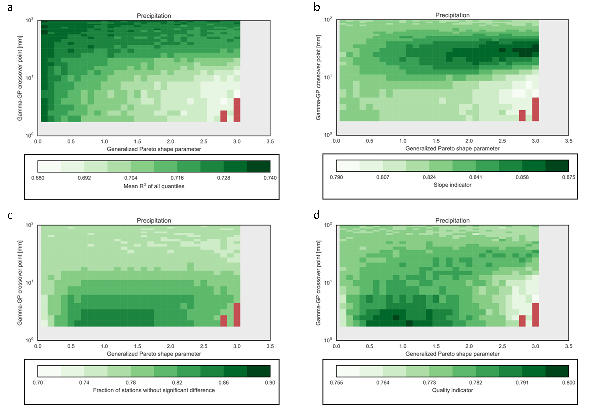
\includegraphics[width=12cm]{figures/sensitivity_results.pdf}
	\caption[Results of the sensitivity analysis]{Results of the sensitivity analysis for the (a) correlation coefficient $R^2$, (b) deviation from a slope of unity, (c) the fraction of significant different station years, (d) the mean of (a) - (c). For the plots in (a) and (b) the mean of the 25th, 50th, 75th, 90th, 95th and 99th percentiles are used. In general, 1 (dark green) is best, 0 (white) is worst. The dark red fields indicate experiments that failed because of a too low threshold and too high GP shape parameter. Note also the logarithmic scale on the y-axis.}
	\label{fig:sens}
\end{figure}


\authorcontribution{JOK conceived the model and analyses, wrote the prototype code and performed preliminary analyses, PS developed and documented the final version of the code (including parameterization), performed all of the final analyses, and okay, something else, created the graphical output. Both authors contributed to the writing of the manuscript}


\begin{subacknowledgements}
	This work was supported by the European Research Council (COEVOLVE, 313797) and the Swiss National Science Foundation (ACACIA, CR10I2\_146314). We thank Shawn Koppenhoefer for assistance compiling and querying the weather databases and Alexis Berne and Grégoire Mariéthoz for helpful suggestions on the analyses. We are grateful to NOAA NCDC and the University of Washingtion for providing free of charge the GHCN-Daily and EECRA databases, respectively.
\end{subacknowledgements}

\end{subappendices}

\printbibliography[heading=subbibintoc]

\end{refsection}
